\documentclass[10pt,a4paper]{article}
\usepackage[utf8]{inputenc} % para poder usar tildes en archivos UTF-8
\usepackage[spanish]{babel} % para que comandos como \today den el resultado en castellano
\usepackage{a4wide} % márgenes un poco más anchos que lo usual
\usepackage[conEntregas]{Sty/caratula}
\usepackage{Sty/mathtools}
\usepackage{Sty/float}
\usepackage[pdftex]{graphicx}
\usepackage{caption}
\usepackage{subcaption}
%\usepackage{Sty/algorithm2e}
\usepackage[ruled,vlined]{Sty/algorithm2e}
%Esto de abajo es para encabezado y pie de pagina
\usepackage{Sty/lastpage}
\usepackage{fancyhdr}
\usepackage{amsfonts}
\usepackage[noend]{algpseudocode}
\usepackage{enumerate} % AGREGO PARA PODER ENUMERAR LAS LINEAS DEL ALGORITMO
\usepackage{wrapfig}


\pagestyle{fancy}
%\fancyhf{} % clear all header and footer fields
%\fancyfoot[R]{\footnotesize Página \thepage\ de \lastpage\}

\cfoot{\thepage /\pageref{LastPage} }

%\newcommand\BlockIf[1]{\KwSty{If} \\ #1 \\ \KwSty{End If}}
\newcommand\BlockElseIf[1]{\KwSty{Else If} \\ #1 \\ \KwSty{End Else If}}
%\newcommand\BlockElse[1]{\KwSty{Else} \\ #1 \\ \KwSty{End Else}}
\newcommand{\Ode}[1]{\hfill O(#1)}
\newcommand{\WhileOde}[1]{\hfill \textit{en el peor caso el ciclo se ejecuta} #1 veces}
\newcommand{\WhileOdeb}[1]{\hfill \textit{el ciclo se ejecuta} #1 veces}
\newcommand{\IfOde}[1]{\hfill \textit{la complejidad de la sentencia del if es de} O(#1)}
\newcommand{\Tde}[1]{\hfill T(#1)}
\begin{document}



\fecha{\today}

\materia{Algoritmos y Estructuras de Datos III}
\titulo{Trabajo Práctico I}
%\grupo{Grupo Numero}

\integrante{Cadaval, Matias}{345/14}{matias.cadaval@gmail.com}
\integrante{Campos Paso, María Candelaria}{774/11}{cande.cp@gmail.com}
\integrante{Lew, Axel Ariel }{225/14}{axel.lew@hotmail.com}
\integrante{Noli Villar, Juan Ignacio}{174/14}{juaninv@outlook.com}

% Pongan cuantos integrantes quieran

\maketitle

\newpage
\tableofcontents		%compilar varias veces si no se actualiza el indice o el pie de pagina

\newpage
\section{Introducción}
En el presente trabajo resolveremos 3 problemas algorítmicos que nos fueron dados, respetando sus requerimientos de complejidad temporal, analizaremos empíricamente los tiempos de ejecución de sus implementaciones, mostraremos un pseudocódigo de los mismos, y las experimentaciones realizadas con sus debidos gráficos.




\section{Problema 1: \textbf{Telégrafo}}
\subsection{Idea general del problema}
Se ha decidido conectar telegráficamente todas las estaciones de un sistema férreo que recorre el país en abanico con origen en la capital (el kilómetro 0). Se nos ofrece cierta cantidad de kilometros de cable para conectar la ciudades de cada ramal. Al ser escaso el presupuesto, se busca lograr conectar la mayor cantidad de ciudades con los metros asignados, sin hacer cortes en el cable. \\
$~~~~~$Se nos propone resolver cuántas ciudades se pueden conectar para cada ramal, con una complejidad de O(n), siendo n la cantidad de estaciones en cada ramal.\\
$~~~~~$Para ello se nos brinda un archivo de entrada, el cual tiene para cada ramal dos líneas: la primera contiene un entero con los kilómetros de cable dedicados al ramal y la segunda los kilometrajes de las estaciones en el ramal sin considerar el 0. Luego de ejecutar nuestro algoritmo, la salida del mismo debe contener, para cada ramal de la entrada, una línea con la cantidad de ciudades conectables encontradas.\\

Un ejemplo de archivo de entrada puede ser, (extracto del archivo Tp1Ej1.in):\\
6 \\
6 8 12 15 \\
35 \\
8 14 20 40 45 54 60 67 74 89 99 \\
100 \\
35 87 141 163 183 252 288 314 356 387 \\
90 \\
6 8 16 19 28 32 37 45 52 60 69 78 82 \\

El mismo indica, en su primer línea que para el ramal 1 tenemos 6km de cable, y en su segunda línea que dicho ramal contiene (además de la capital, implícita, en el kilómetro 0) una estación en el kilómetro 6, otra en el 8, otra en el 12 y la última en el kilómetro 15. Luego para el ramal 2, tenemos 35 kilómetros de cable, y estaciones en los kilómetros: 8 14 20 40 45 54 60 67 74 89 y 99. Así sucesivamente para el resto de los ramales.\\
$~~~~~$El archivo de salida luego de ejecutarse nuestro algoritmo deberá ser de la siguiente pinta, (extracto del archivo Tp1Ej1.out):\\
3 \\
6 \\
4 \\
14 \\

Este último archivo indica la cantidad de ciudades que se pueden conectar para cada ramal. En el caso del ramal 1, para el cual se tienen 6km de cable disponibles, y contiene ciudades en los kilómetros: 0 6 8 12 15 vemos que la solución debería ser que se pueden conectar como máximo 3 ciudades, a continuación explicaremos cómo se deduce esto.\\

Si conectamos la capital con la ciudad del kilómetro 6, al tener sólo 6km de cable, nuestra solución sería que pudimos conectar sólo 2 ciudades. Pero como debemos maximizar esta cantidad, podemos ver que si en vez de conectar a la capital con la primer estación del ramal, conectamos la ciudad del kilómetro 6, con su siguiente y con la del kilómetro 12, entonces como entre el kilómetro 6 y el 8 hay una diferencia de 2kms y entre el 8 y el 12 una diferencia de 4kms, vemos que la máxima cantidad de estaciones conectadas con 6km de cable para el ramal 1, es 3. La misma lógica se la aplica para los ramales restantes.\\

\subsection{Explicación y pseudocódigo}

El algoritmo empieza ubicando dos índices llamados ``start" $ $y ``actual" $ $ en la primera ciudad e inicializando ``restemp" $ $ con el valor 0 (a lo largo del algoritmo esta variable contendrá la solución parcial del ejercicio). Luego, si el cable es suficientemente largo, avanza ``actual"$ $ hasta la segunda ciudad, y le resta al cable esa distancia (entre la primer ciudad y la segunda). Cada vez que una nueva ciudad es conectada, la variable ``conectadas" $ $ aumenta en uno, al igual que el índice ``actual"$ $. De esta manera, continúa (restando la distancia entre la tercera y la segunda, luego entre la cuarta y la tercera, etc.) hasta que ya no se puedan conectar más ciudades, es decir, hasta que el cable se acaba, o en caso de llegar a la última ciudad (cuando ``actual"$ $ apunta a la última ciudad).  Si llegamos a la última ciudad, el algoritmo verifica si la cantidad de ciudades del ramal recién calculado (es decir, ``conectadas" $ $) es mayor que ``restemp" $ $; lo reemplaza en caso de que si, y retorna ``restemp" $ $, que es el resultado final. En caso de que el cable se acabe, calcula la distancia entre la ciudad apuntada por ``start" $ $ y la siguiente ciudad; suma esa distancia al resto del cable que quedo disponible y avanza el índice ``start" $ $ a la siguiente ciudad del ramal, para ver si se puede construir otra conexión con una mayor cantidad de ciudades. Además, verifica si ``conectadas" $ $ es mayor que ``restemp" $ $, lo reemplaza en caso positivo, y luego le resta uno a dicha variable (siempre que esta sea mayor a 0), pues esto simboliza que una ciudad fue desconetada. Con esta nueva cantidad de cable disponible, los pasos recien descriptos se repiten, y se verifica nuevamente si se puede incluir la ciudad siguiente (la siguiente a ``actual"$ $) al ramal. El algoritmo finaliza una vez que se llegue a la última ciudad.

A continuación mostramos un pseudocódigo de la implementación explicada anteriormente. \\

int conectar(vector$<$int$>$ v , int cable) \{ \\
$~~~~~~~~~~~~$int resTemp $\leftarrow$ 0 \Ode{1}\\
$~~~~~~~~~~~~$int start $\leftarrow$ 0 \Ode{1}\\
$~~~~~~~~~~~~$int actual $\leftarrow$ 0 \Ode{1}\\
$~~~~~~~~~~~~$int aux $\leftarrow$ 0 \Ode{1}\\
$~~~~~~~~~~~~$\textbf{mientras} (actual no apunte al último elemento del vector) \{   \Ode{n} \\
$~~~~~~~~~~~~~~~$\textbf{mientras}(cable $\geq$ 0 y actual no apunte al ultimo elemento del vector) \{  \Ode{cable} \\
$~~~~~~~~~~~~~~~~~~~~$Guardamos en aux el cable, por si este pasa a ser negativo \Ode{1}\\
$~~~~~~~~~~~~~~~~~~~~$Le restamos al cable la distancia entre lo apuntado por actual y su siguiente; \Ode{1}\\
$~~~~~~~~~~~~~~~~~~~~$\textbf{si} (longitud del cable $\geq$ 0) \{  \Ode{1}\\
$~~~~~~~~~~~~~~~~~~~~~~~~~~$Incrementamos conectadas en 1 y avanzamos el puntero actual \Ode{1}
$~~~~~~~~~~~~~~~~~~~~$\} \\
$~~~~~~~~~~~~~~~~~~~~$Si conectadas es igual a uno se lo cambia por dos;  \Ode{1}\\
$~~~~~~~~~~~~~~~~$\}\\
$~~~~~~~~~~~~~~~$Si el cable en negativo, se actualiza su valor por el de aux\\
$~~~~~~~~~~~~~~~~~~$Si conectadas es mayor que restemp se actualiza el valor de restemp por el de conectadas\\
$~~~~~~~~~~~~~~~$\textbf{si}(resTemp == 0) \{  \Ode{1} \\
$~~~~~~~~~~~~~~~~~~~~$Conectadas  $\leftarrow$ 0; \Ode{1}\\
$~~~~~~~~~~~~~~~~~~~~$Avanzamos los dos índices, start y actual;  \Ode{1}\\
$~~~~~~~~~~~~~~~$\} \textbf{si no} \{ \\
$~~~~~~~~~~~~~~~~~~~~$Decrementamos conectadas en 1, ya que desconectamos la primer ciudad \\
$~~~~~~~~~~~~~~~~~~~~$Sumamos al cable la distancia entre lo apuntado por start y su siguiente;\de{1}\\
$~~~~~~~~~~~~~~~~~~~~$Incrementamos start en 1;  \Ode{1}\\
$~~~~~~~~~~~~~~~$\} \\
$~~~~~~~~~~~~$\} \\
$~~~~~~~~~~~~$Devolvemos restemp, en caso de que sea uno, se cambia su valor por dos; \Ode{1} \\
\}\\

\subsection{Deducción de la cota de complejidad temporal y correctitud}

A partir del siguiente análisis de nuestro algoritmo, deducimos que la complejidad del mismo para resolver el problema dado es de O(n) en el peor de los casos, donde n es la cantidad de estaciones en cada ramal. \\

El algoritmo que construimos consta de dos ciclos: el primero se ejecuta a lo sumo n veces, y eso ocurre cuando tenemos un cable demasiado corto que no alcanza para unir ni siquiera dos ciudades. Lo que ocurre en este caso, es que los dos índices (``start"$ $ y ``actual"$ $) se van incrementando en uno, recorriendo así todo el vector cada índice, y el segundo ciclo solo iteraría una vez pues el cable pasaría a ser negativo instantaneamente. También podría ocurrir que el primer while se ejecutarse solo una vez (si se da un cable muy largo); en este caso el segundo while es el que iteraría n veces, llevando el puntero ``actual"$ $ hasta el final, pero sin mover ``start"$ $ por lo que seria considerado como el mejor caso, aunque este también tiene una complejidad O(n).\\

En otros casos, el segundo while del algoritmo se ejecuta mientras que la longitud del cable sea positiva y el índice ``actual"$ $ no apunte a la última ciudad; este ciclo va sumando ciudades al ramal y guarda cuántas ciudades se conectaron. Mientras que va conectando ciudades, el algoritmo hace avanzar el segundo índice (``actual"$ $) y, cuando el cable pasa a ser negativo, se incrementa el primer índice ``start"$ $, se suma esa diferencia al cable, se verifica si hay que actualizar el resultado, y vuelve a comenzar el segundo ciclo. Este proceso continúa hasta que ``actual"$ $ alcance a la última ciudad. Notar que en cada iteración, ``actual"$ $ no siempre avanza, y cuando no lo hace, ``start"$ $ sí. Si ocurre que ``start"$ $ y ``actual"$ $ se superponen, entonces en la iteración siguiente, si ``start"$ $ vuelve a avanzar, lo empuja(es decir, ``actual"$ $ también avanza). Aquí se puede obervar el peor caso, que ocurre cuando ``actual"$ $ llega hasta cierto punto arbitrario, y luego ``start"$ $ lo alcanza. Si esto ocurre constantemenete, se recorre linealmente el vector dos veces, y aunque sigue siendo O(n), es el caso que más iteraciones produce y por eso es considerado el peor caso.\\

El algoritmo termina una vez que el segundo puntero llega al final. Como ninguno de los dos índices retrocede nunca, y si ``start"$ $ alcanza a ``actual"$ $, en la siguiente iteración ``actual"$ $ avanza,  se puede deducir que el algortimo es lineal y por lo tanto tiene una complejidad O(n). Por esta razón decimos que nuestro algoritmo es correcto, ya que siempre llega al final, siempre devuelve el resultado esperado y respeta la cota del enunciado. \\

Las funciones que usamos: $>$, $<$, $\geq$, $+$, $-$, $==$, tienen complejidad constante al igual que las asignaciones. También sabemos por la documentación de C++, que el $operator[]$ del vector es de complejidad O(1) al igual que la función del vector $.back()$.\\

\subsection{Casos de test, experimentación, y gráficos}

\subsubsection{Caso random}
Vamos a mostrar la implementación de un test generado sin ninguna intencionalidad, pero antes explicaremos como fue creado. \\

Implementamos una función que genera números random para el archivo que le vamos a pasar por entrada a nuestro algoritmo con los siguientes criterios:
\begin{itemize}
\item Elegimos en este ejemplo que el primer ramal iba a contar con una estación, el segundo con 101, el tercero con 201 y asi sumando de a 100.
\item Para el valor de la longitud de cable disponible de cada ramal, decidimos que sea un número random entre 1 y la cantidad de estaciones de cada ramal.
\item Para los kilometrajes de las estaciones tuvimos en cuenta, que estos debían estar ordenados de menor a mayor, sin contener el kilómetro 0. 

El archivo que contiene dicha función se puede encontrar en la carpeta Ejercicio 1, y se llama: generadorArchivosInRandom.py.

\end{itemize}

Una vez que generamos el archivo del input con dicho test, ejecutamos nuestro algoritmo obteniendo el archivo de salida con la cantidad de ciudades conectadas para cada ramal, e imprimimos por pantalla el tiempo promedio de 100 corridas de nuestro algoritmo, en milisegundos. Este es el tiempo que tarda en calcular la máxima cantidad de estaciones conectadas de cada ramal. Decidimos calcular el tiempo promedio porque al ejecutarlo un par de veces nos dimos cuenta que el tiempo varía aunque resuelva la misma instancia, entonces decidimos correrlo una cierta cantidad de iteraciones (en este caso 100), e ir acumulando los tiempos para luego dividir este acumulador por 100 y así obtener un valor promedio de los tiempos en los que se tarda en resolver el problema para cada ramal. \\

Con estos tiempos creamos el gráfico de la figura \ref{ej1-random} que mostramos a continuación, en el que hacemos una comparación con la gráfica de O(n) y observamos como nuestro algoritmo cumple dicha complejidad.

\begin{figure}[H]
\begin{center}

\minipage{0.8\textwidth}
  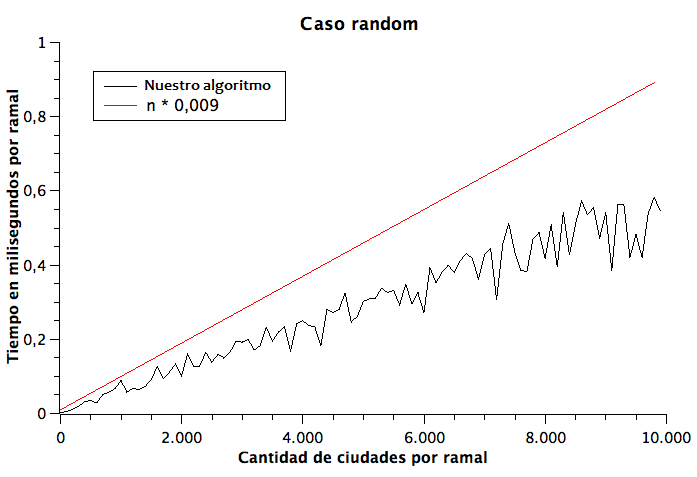
\includegraphics[width=\linewidth]{../graficos/ej1/CasoRandom.png}
  \caption{{\small Comparación con O(n). Dado un archivo de entrada con longitud de cable y kilometrajes de estaciones random.}} \label{ej1-random}
\endminipage

\end{center}
\end{figure}


\subsubsection{Peor caso}

El próximo test generado consiste en tener una ciudad al final muy lejos, lo que produciría que ``actual" $ $ llegue hasta el anteúltimo, luego ``start" $ $  lo alcance y esto produzca que se pase por todas las ciudades dos veces. Esto lo consideramos un Peor caso ya que para el resto de los casos no hace falta pasar dos veces por todas las ciudades.  Para probar esto, escribimos un script que nos asegura que la última ciudad este muy alejada. En cuanto a las estaciones del ramal, configuramos números random y el ultimo muy grande. Estos archivos se encuentran en la carpeta ``Ejercicio 1" $ $ con prefijo ``5toEjemplo" $ $, y``generadorArchivosInRandom.py" $ $es el script con los distintos tests, comentados. Veamos un ejemplo:\\

\begin{itemize}
\item La longitud del cable llega hasta la anteúltima ciudad, y la última ciudad esta muy lejos:\\
\textbf{in:}\\
90\\
3 6 8 12 15 20 24 49 58 70 90 1000 \\
\textbf{out:}\\
12\\

En este caso la longitud del cable es 90, por lo tanto está bien que nuestro algoritmo devuelva que conectó 12 ciudades.\\
\end{itemize}

\begin{figure}[H]
\begin{center}

\minipage{0.8\textwidth}
  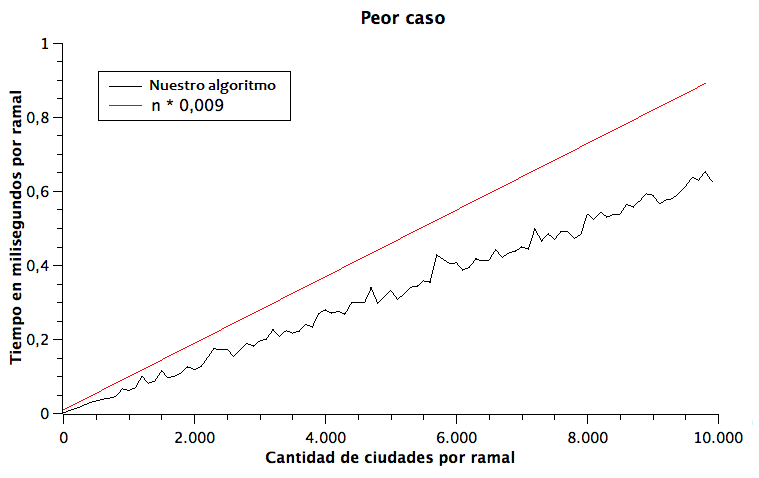
\includegraphics[width=\linewidth]{../graficos/ej1/PeorCaso.png}
  \caption{{\small Comparación con O(n). Dado un archivo de entrada con un cable suficientemente largo como para llegar a la anteúltima ciudad pero con una última ciudad muy lejana, lo que genera que se avancen los dos índices.}} \label{ej1-peor}
\endminipage

\end{center}
\end{figure}

En la figura \ref{ej1-peor} vemos como nuestro algoritmo sigue respentando el límite de complejidad propuesto por la cátedra, a pesar de que éste sea un caso ``border" $ $. \\

\subsubsection{Mejor caso}

Otro test que decidimos hacer fue el que la longitud del cable es tan larga que permite conectar todas las ciudades de los ramales. Esto lo consideramos como el mejor caso, ya que al tener un cable suficientemente largo como para conectar todas las ciudades, el primer puntero ($"$start$"$) no es necesario que se mueva, solo avanza el segundo. Para ver esto , escribimos un script de manera tal que la cantidad de kilómetros de cable siempre supere la distancia entre la primera ciudad y la ciudad del último kilómetro del ramal. Al medir los tiempos promedios vemos que nuestro algoritmo sigue tardando menos que O(n), y lo podemos observar en la figura que sigue, pero antes veamos un ejemplo. \\

\begin{itemize}
\item El cable alcanza para conectar todas las ciudades:\\
\textbf{in:}\\
10000\\
1 4 67 78 90 95 120 150 270 380 456 900 1300 1809 5546 8403\\
\textbf{out:}\\
17\\
\end{itemize}
En este caso al tener un cable de longitud = 10000km y todas las estaciones estar a distancia menor que 10000km, el algoritmo devuelve 17 que son la cantidad de estaciones del ramal + la ciudad de kilómetro 0, pues la distancia entre ésta ciudad y la primera es de 1km. Veamos el gráfico \ref{ej1-mejor}. \\

\begin{figure}[H]
\begin{center}

\minipage{0.8\textwidth}
  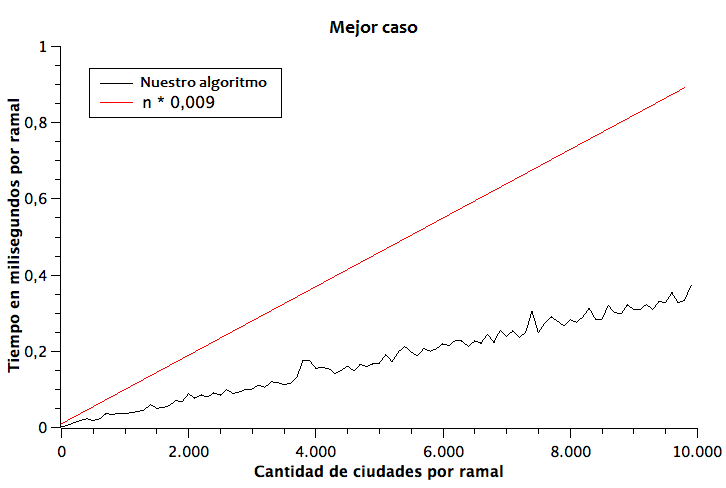
\includegraphics[width=\linewidth]{../graficos/ej1/MejorCaso.png}
  \caption{{\small Comparación con O(n). Dado un archivo de entrada con un cable muy largo y kilometrajes de estaciones random.}} \label{ej1-mejor}
\endminipage

\end{center}
\end{figure}

\subsubsection{Mejor caso vs Caso random vs Peor caso vs O(n)}

A continuación ilustramos un gráfico (figura \ref{ej1-todos}) en donde comparamos el tiempo que tarda el algoritmo en el mejor caso, en el caso randon, y en el tiempo del peor caso, y con O(n). Para realizar el gráfico definimos la línea O(n) como n $*$ 0,009.

\begin{figure}[H]
\begin{center}

\minipage{0.8\textwidth}
  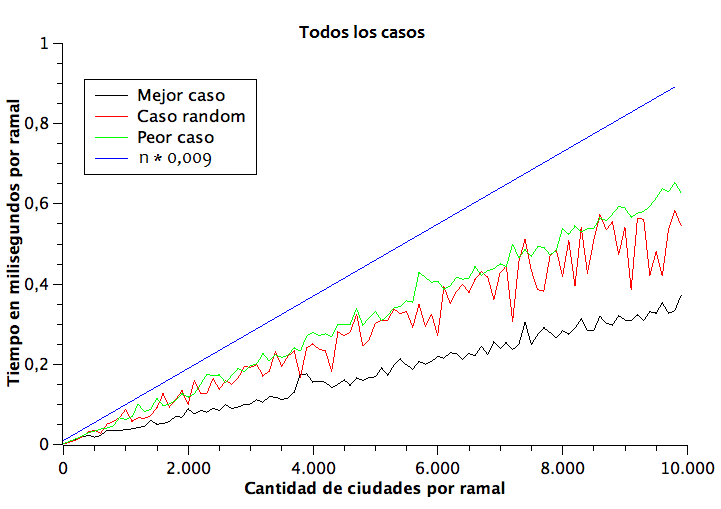
\includegraphics[width=\linewidth]{../graficos/ej1/TodosLosCasos.png}
  \caption{{\small Comparación con O(n) del mejor, peor y caso random anteriormente explicados. }} \label{ej1-todos}
\endminipage

\end{center}
\end{figure}


\subsubsection{Otros casos interesantes}
\begin{itemize}
\item Cuando el cable alcanza para conectar solo las primeras ciudades:\\
\textbf{in:}\\
9\\
1 2 3 4 5 40 55 68 79 99 130 139 200 259 2889\\
\textbf{out:}\\
6\\

\end{itemize}

Al tener un cable de longitud 9km, las primeras 5 estaciones estar a 1 kilómetro de distancia entre ellas, y las siguientes distancias superar los 9km, si contamos estas 5, y a la ciudad del kilómetro 0, no devuelve las 6 ciudades que conecta.\\

\begin{figure}[H]
\begin{center}

\minipage{0.8\textwidth}
  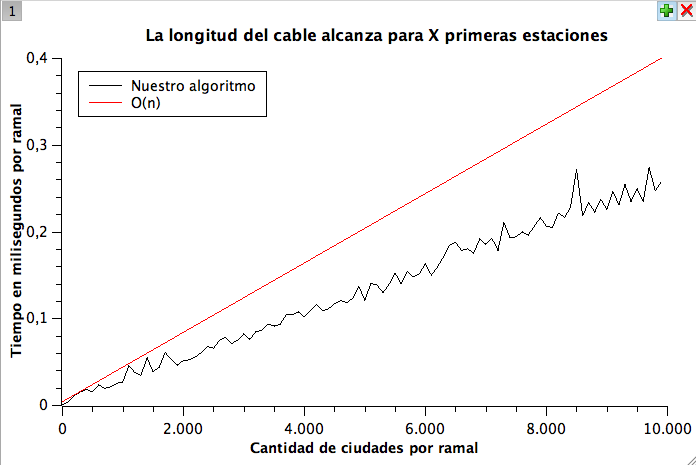
\includegraphics[width=\linewidth]{../graficos/ej1/PrimerasCiudades.png}
  \caption{{\small Comparación con O(n). Dado un archivo de entrada donde entre las primeras ciudades hay una distancia corta.}} \label{ej1-primerasciudades}
\endminipage

\end{center}
\end{figure}

\begin{itemize}
\item Cuando el cable no alcanza y no se conectan ciudades:\\
\textbf{in:}\\ 
1\\
4 8 12 16 20 24 28 32 \\
\textbf{out:}\\
0\\

La distancia entre todas las estaciones es de más de 1km, y el cable tiene un largo de 1km, por lo tanto, al faltarle siempre cable para poder conectar al menos dos ciudades, devuelve 0. Esto es correcto ya que no alcanza el cable y no ``conecta" $ $ ciudades. \\

A continuación mostramos el gráfico \ref{ej1-cablecorto} que resulta de medir el tiempo que tarda el algoritmo al correr un archivo de entrada que generamos con ciudades que están a una distancia mayor a un, con un cable de longitud 1 y compararlo con O(n), en particular para este ejemplo, lo comparamos con 0,009 $*$ n. Los archivos que usamos son: ``generadorArchivosInRandom.py" $ $ (ejemplo 6), ``2doEjemploTiempoMilisegundos.txt"  $ $, \\ ``2doEjemploCableCorto.in"  $ $, ``2doEjemploCableCorto.out"  $ $ y , ``ejemploTamCiudades.txt"  $ $.\\

\end{itemize}

\begin{figure}[H]
\begin{center}

\minipage{0.8\textwidth}
  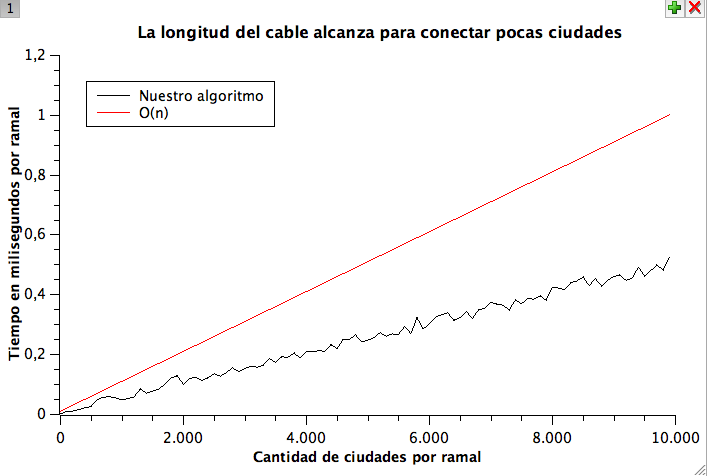
\includegraphics[width=\linewidth]{../graficos/ej1/CableCorto.png}
  \caption{{\small Comparación con O(n). Dado un archivo de entrada donde se da un cable corto para conectar las ciudades.}} \label{ej1-cablecorto}
\endminipage

\end{center}
\end{figure}



\newpage
\section{Problema 2: \textbf{A Medias}}
\subsection{Idea general del problema}
Se nos propone realizar un algoritmo en el que dados n número enteros en cualquier orden se debe devolver otros n números, donde el i-ésimo de ellos represente la parte entera de la mediana de los primeros i números de la entrada.
La mediana de un conjunto ordenado de n números se define como x$_{(n+1)/2}$ si n es impar, o como (x$_{n/2}$ + x$_{n/2+1)}$)/2  si n es par.
Un ejemplo de entrada puede ser: \\
\\
2 7 2 8 4 9 1 6 5 \\
\\
Su salida deberia ser: \\
\\
2 4 2 4 4 5 4 5 5

\subsection{Explicación, correctitud y pseudocódigo}

Lo que hicimos fue dividir un arreglo (L) de tamaño n en dos conjuntos (multiconjuntos, ie: pueden tener repetidos), uno con los elementos menores a cierto número (A) y otro con los mayores (B). Los elementos iguales a ese número pueden ir en cualquiera de los dos. Entonces sabemos que, si ordenaramos el arreglo, L[ \textbar A\textbar] = max(A) y L[\textbar A\textbar+1] = min(B). Tres casos importantes: 

\begin{itemize}
\item Si ambos conjuntos tienen la misma cantidad de elementos entonces L[\textbar A\textbar] = L[n/2] = max(A) y L[n/2+1] = min(B). Entonces la mediana(L) = (max(A)+min(B))/2
\item Si \textbar A\textbar = \textbar B\textbar + 1 (n es impar), entonces L[(n+1)/2] = max(A). Entonces la mediana(L) = max(A)
\item Si \textbar A\textbar + 1 = \textbar B\textbar (n es impar), entonces L[(n+1)/2] = min(B). Entonces la mediana(L) = min(B)
\end{itemize}


Nuestro algoritmo lo que hace es: 
\begin{itemize}
\item Si el arreglo original no contiene elementos, entonces devolvemos un vector vacio
\item Insertar el primer elemento en el conjunto de los elementos más grandes (B) e insertarlo también en la posición 1 del resultado, ya que es mediana.
\item Hasta que no queden elementos en el arreglo original, se agrega el elemento i del arreglo original en el conjunto A si es menor a la mediana del paso anterior y al conjunto B si es mayor. Si la diferencia entre la cantidad de elementos de ambos conjuntos es igual a 2, entonces quitamos el mayor elemento de A o el menor elemento de B y lo insertamos en el otro para que nos queden dos conjuntos de igual tamaño. Entonces podemos utilizar la propiedad de arriba y sacar fácilmente la mediana, obteniendo el máximo y/o mínimo de los conjuntos correspondientes. Ponemos la mediana en la posición i del resultado y avanzamos a la siguiente iteración.
\end{itemize}

A continuación mostraremos su pseudocódigo y deduciremos su complejidad: \\
--------------------------------------------------------------------------------------------------------------\\
vector$<$int$>$ medianas(vector$<$int$>$ a)\{ \\
$~~~~~~~~~~~~~$\textbf{si} (a es vacio) \{ \\ \IfOde{1}\\
$~~~~~~~~~~~~~~~~~~$devolvemos un vector vacio \Ode{1}\\
$~~~~~~~~$\} \\
$~~~~~~~~$creamos el vector res de tamaño igual que a, inicializado con ceros\Ode{tamaño de a} \\
$~~~~~~~~$res[0] $\leftarrow$ a[0]\Ode{1} \\
$~~~~~~~~$creamos el multiset vacío: masGrandes \Ode{1} \\
$~~~~~~~~$creamos el multiset vacío: masChicos \Ode{1} \\
$~~~~~~~~$int mínimo\Ode{1} \\
$~~~~~~~~$int máximo\Ode{1} \\
$~~~~~~~~$insertamos a masGrandes el primer elemento del vector \Ode{log(tamaño de masGrandes)} = \Ode{1} \\
$~~~~~~~~$ \textbf{para cada} (int i = 1; i $<$ al tamaño de a; i++)\{ \\ \WhileOdeb{tamaño de a} \\
$~~~~~~~~~~~~~$\textbf{si} (el elemento i de a $\geq$ el elemento i-1 de res)\{ \\ \IfOde{1} \\
$~~~~~~~~~~~~~~~~~~$insertamos a masGrandes el elemento i de a \Ode{log(tamaño de masGrandes)} \\
$~~~~~~~~~~~~~$ \} \textbf{si no} \{ \\
$~~~~~~~~~~~~~~~~~~$ lo insertamos en masChicos \Ode{log(tamaño de masChicos)} \\
$~~~~~~~~~~~~~$ \} \\
$~~~~~~~~~~~~~$\textbf{si} (el tamaño de masGrandes - tamaño de masChicos == 2) \{ \\ \IfOde{1}\\
$~~~~~~~~~~~~~~~~~~$minimo $\leftarrow$ $\ast$ masGrandes.begin() \Ode{1}\\
$~~~~~~~~~~~~~~~~~~$borramos mínimo de masGrandes  \Ode{log(tamaño de masGrandes)} \\
$~~~~~~~~~~~~~~~~~~$insertamos minimo a masChicos \Ode{log(tamaño de masChicos)} \\
$~~~~~~~~~~~~~$\} \textbf{si no, si}(el tamaño de masGrandes - tamaño de masChicos == -2) \{ \\ \IfOde{1}\\
$~~~~~~~~~~~~~~~~~~$maximo $\leftarrow$ $\ast$ masChicos.rbegin() \Ode{1}\\
$~~~~~~~~~~~~~~~~~~$borramos máximo de masChicos \Ode{log(tamaño de masChicos)} \\
$~~~~~~~~~~~~~~~~~~$insertamos máximo a masGrandes \Ode{log(tamaño de masGrandes)} \\
$~~~~~~~~~~~~~$\} \\
$~~~~~~~~~~~~~$\textbf{si} (el tamaño de masGrandes == el tamaño de masChicos) \{ \\ \IfOde{1}\\
$~~~~~~~~~~~~~~~~~~$minimo $\leftarrow$ $\ast$ masGrandes.begin() \Ode{1}\\
$~~~~~~~~~~~~~~~~~~$maximo $\leftarrow$ $\ast$ masChicos.rbegin() \Ode{1}\\
$~~~~~~~~~~~~~~~~~~$posicion i de res $\leftarrow$ (maximo + minimo)/2; \Ode{1}\\
$~~~~~~~~~~~~~$\} \textbf{si no, si} (el tamaño de masGrandes - el tamaño de masChicos == 1) \{ \\ \IfOde{1}\\
$~~~~~~~~~~~~~~~~~~$minimo $\leftarrow$ $\ast$ masGrandes.begin() \Ode{1} \\
$~~~~~~~~~~~~~~~~~~$posición i de res $\leftarrow$  minimo \Ode{1} \\
$~~~~~~~~~~~~~$\} \textbf{si no, si} (el tamaño de masGrandes - tamaño de masChicos == -1) \{ \\ \IfOde{1}\\
$~~~~~~~~~~~~~~~~~~$maximo $\leftarrow$ $\ast$ masChicos.rbegin() \Ode{1}\\
$~~~~~~~~~~~~~~~~~~$posición i de res $\leftarrow$ maximo \Ode{1}\\
$~~~~~~~~~~~~~$\} \\
$~~~~~~~~$\} \\
$~~~~~~~~$devolvemos res \Ode{1}\\
\} \\
------------------------------------------------------------------------------------------------------------\\

\subsection{Deducción de la cota de complejidad temporal}
Los conjuntos utilizados son  \textbf{$<$multiset$>$} cortesía de C++. La inserción y borrado cuesta O(log(n)) siendo n la cantidad de elementos del conjunto, ya que usamos las funciones de C++: \textbf{insert} y \textbf{erase} de los \textbf{multisets}, respectivamente. La función \textbf{erase} cuesta O(log(n)) + O(m) siendo n = cantidad de elementos del conjunto, y m el número de elementos eliminados, en nuestro caso, siempre es uno porque llamamos a erase una vez con el elemento mínimo y otra con el máximo.\\
Obtener máximo y mínimo nos cuesta O(1), pues usamos \textbf{begin()} y \textbf{rbegin()} de complejidad constante. Además usamos la función \textbf{size} de los \textbf{multisets} de complejidad constante. \\ 

Tenemos como entrada un vector de tamaño n. Los pasos a realizar son: \\

1) Crear el vector donde se guardará y devolverá el resultado: se realiza en O(n). \\

2) Insertar el primer elemento del arreglo original en el arreglo resultado es O(1), porque usamos \textbf{operator[]} de complejidad constante. \\

3) Luego, se realizan n-1 iteraciones, en las cuales: \\
\begin{itemize}
\item Se realiza una comparación O(1) y se hace una inserción en alguno de los conjuntos en O(log(n)).
\item Si la diferencia entre la cantidad de elementos de ambos conjuntos es igual a 2, se elimina el mayor elemento de A o el menor elemento de B en O(log(n)) y lo insertamos en el otro en O(log(n)).
\item Obtenemos el máximo y/o mínimo de los conjuntos correspondientes para calcular la mediana y la insertamos en el resultado en O(1).
\end{itemize}
Aclaración: en este ciclo, en realidad, las complejidades no son O(log(n)) sino que son O(log(i)) siendo i el número de iteración. Pero como i $<$ n $\forall$ i, entonces lo acotamos por O(log(n)). \\

Entonces la complejidad total del algoritmo es O(n + (n-1)log(n)) = O(n log(n)).

\subsection{Casos de test y sus gráficos}
Vamos a analizar los tiempos de nuestro algoritmo para entradas de distinto tamaño, divididos en tres casos (todos O(n log n)):
\begin{itemize}
\item Peor caso: Corresponde al caso donde en la mitad de las iteraciones del ciclo, la diferecia entre la cantidad de elementos entre los conjuntos masGrandes y masChicos es igual a dos. Entonces hay que realizar en cada una de estas un borrado y una insercion. No existe peor caso que este, ya que al realizar una insercion y borrado, los conjuntos quedan con la misma cantidad de elementos y se necesitan dos iteraciones mas ciclo para tener que volver a reacomodar los elementos. Entradas crecientes y decrecientes son ejemplos de peor caso, que es lo que utilizaremos
\item Mejor caso: Resulta cuando en ninguna iteracion la diferecia entre la cantidad de elementos entre los dos conjuntos es igual a dos, y no hay que hacer borrado e insercion. Para que pase esto, nuestra entrada consistira en una cadena de numeros, donde la subcadena de numeros en posicion par es creciente, y la subacadena de numeros en posicion impar es decreciente 
\item Caso random: Utilizando la funcion random de python, generamos entradas al azar de diferentes entradas
\end{itemize}
Los tiempos se miden de la misma forma que en el ejercicio 1. Cantidad representa la cantidad de numeros pasados como parametro y el tiempo se mide en milisegundos
\begin{figure}[H]
\begin{center}

\minipage{0.8\textwidth}
  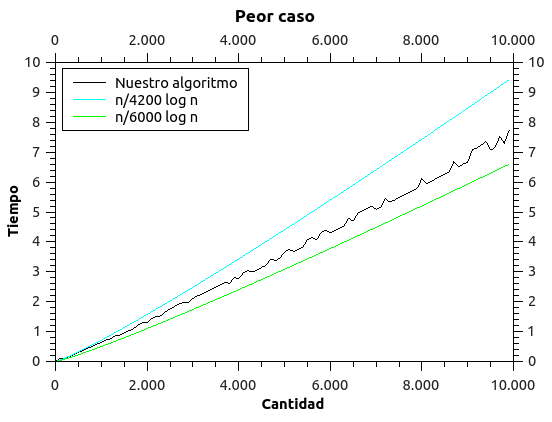
\includegraphics[width=\linewidth]{../graficos/ej2/Peor.png}
  \caption{{\small Comparación del peor caso con O((n/6000)log(n)) y O((n/4200)log(n)).}} \label{ej2-peor-caso}
\endminipage

\end{center}
\end{figure}


\begin{figure}[H]
\begin{center}

\minipage{0.8\textwidth}
  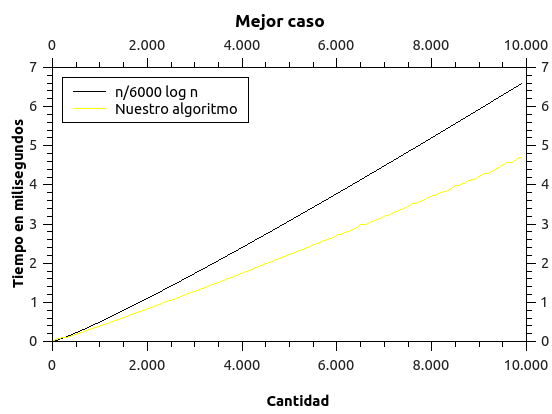
\includegraphics[width=\linewidth]{../graficos/ej2/Mejor.png}
  \caption{{\small Comparación del mejor caso con O((n/6000)log(n)).}} \label{ej2-mejor-caso}
\endminipage

\end{center}
\end{figure}


\begin{figure}[H]
\begin{center}

\minipage{0.8\textwidth}
  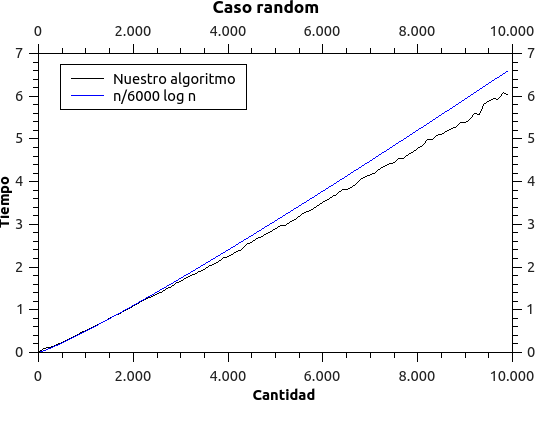
\includegraphics[width=\linewidth]{../graficos/ej2/Random.png}
  \caption{{\small Comparación de un caso random con O((n/6000)log(n)).}} \label{ej2-random-caso}
\endminipage

\end{center}
\end{figure}

\begin{figure}[H]
\begin{center}

\minipage{0.8\textwidth}
  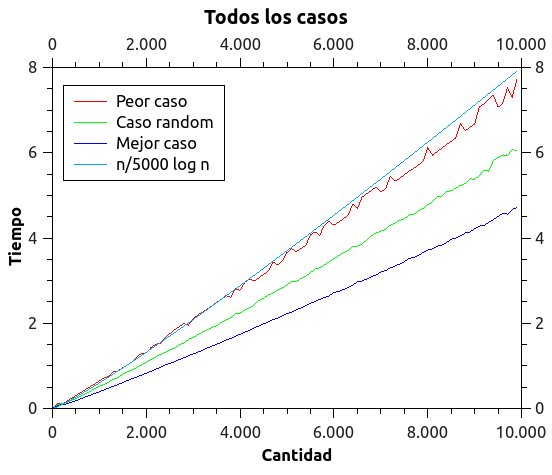
\includegraphics[width=\linewidth]{../graficos/ej2/Todos.png}
  \caption{{\small Comparación de los tres casos anteriores con O((n/5000)log(n)).}} \label{ej2-todos-casos}
\endminipage

\end{center}
\end{figure}


\newpage
\section{Problema 3: \textbf{Girls Scouts}}
\subsection{Idea general del problema}
El ejercicio nos propone diseñar un algoritmo para resolver el siguiente problema: dado un grupo de exploradoras, y el conjunto 
de amigas de cada una de ellas, organizar una ronda de manera tal que exista la menor distancia posible entre cada amistad, es 
decir, minimizar la suma de las distancias entre todos los pares de amigas.\\
La complejidad de la solución debe ser estrictamente menor que O(e$^e$.a$^2$), donde ``e"$ $ es la cantidad de exploradoras en cada grupo, y ``a"$ $ la cantidad de amistades. \\

Algunos ejemplos de posibles datos de entrada del problema son: \\
a bcde;b acde;c abde;d abc;e abc \\
a bcd;b ae;c ad;d ac;e b \\
a fb;b gc;d gc;f agh;e hd \\
x yz \\

Cada línea corresponde a un grupo de exploradoras; y se compone de una exploradora, seguida por una sucesion de amistades
separadas por ``;"$ $. Por ejemplo, en la primer línea, el grupo de exploradoras esta compuesto por ``a"$ $ cuyas amigas son [bcde],
``b"$ $ con [acde], ``c"$ $ con [abde] y por último ``d"$ $ y ``e"$ $ con  [abc]. Asumimos que las amistades son simétricas, es decir, si ``
a"$ $ es amiga de ``b"$ $, entonces ``b"$ $ es amiga de ``a"$ $. Por lo tanto, aunque ocurra que ``x"$ $ este en el conjunto de amigas 
de ``y"$ $, pero ``y"$ $ no este en el de ``x"$ $, debemos interpretarlo como que cada una esta en el grupo de amigas de la otra.  \\

Las salidas que corresponden a los ejemplos recien dados son las siguientes (mismo orden): \\
2 abdce \\
2 abecd \\
3 abgcdehf \\
1 xyz \\

La sucesión de caracteres representa la solución del problema, es decir, la ronda en la que exista la menor distancia posible entre cada 
amistad. El número que está delante, es la máxima distancia que hay entre dos amigas en la ronda solución. Si es que existe mas de una 
ronda óptima, se debe dar la que esté primera alfabéticamente. 

\subsection{Explicación y pseudocódigo}
Para resolver el problema diseñamos un algoritmo que consiste en, dado un grupo de exploradoras, generar todas las rondas 
posibles, e ir almacenando aquella que hasta el momento es la ``mejor"$ $ entre las ya calculadas (con ``mejor"$ $ nos referimos a 
aquella que minimiza la suma de las distancias entre amigas).\\

Para armar las permutaciones, construimos la funcion $permutar$. Mediante esta funcion vamos generando todas las rondas posibles, 
pues cada vez que la llamamos, genera la siguiente permutacion (siguiente en orden alfabético) de la ronda, hasta que ya no hayan 
nuevas. Su algoritmo consiste en buscar el mayor índice k tal que a[k] $<$ a[k+1]; luego buscar el mayor índice i tal que a[k] $<
$ a[i]; swapear a[k] con a[i]; y por último aplicar reverso a partir del elemento k (sin incluirlo) hasta el final de la lista. Entonces, a medida 
que vamos armando las distintas rondas posibles, calculamos la suma de distancias y luego la comparamos con la suma de la que 
tenemos almacenada. Si la suma de la nueva ronda es menor entonces nos guardamos la nueva, pues es ``mejor"$ $ que la que 
teníamos. Caso contrario, pasamos a calcular la siguiente ronda, pues si la suma es mayor esa ronda no nos interesa, y si es igual 
tampoco, porque como las rondas se van calculando en orden alfabetico, entonces la que ya tenemos guardada va a estar primera 
teniendo en cuenta dicho orden. \\

El algoritmo termina una vez que se hayan calculado todas las rondas posibles. La última ronda que quedó guardada va a ser nuestra 
solución. Por otra parte, la máxima distancia entre dos amigas de la ronda, se calcula en simultáneo con la suma de las distancias, y 
siempre la almacenamos junto con la ``mejor"$ $ ronda durante todo el algoritmo. \\

Para entender mejor la idea dejamos el algoritmo en pseudocódigo:\\   
--------------------------------------------------------------------------------------------------------------\\
mejorRonda (dado un conjunto de exploradoras (exp) y sus amistades) \\
$~~~~~~~~$crear int sumaMinima \\
$~~~~~~~~$crear int maxDist \\
$~~~~~~~~$crear Ronda rondaOptima  \\
$~~~~~~~~$ordenar alfabeticamente exp \\
$~~~~~~~~$rondaOptima $\leftarrow$ exp \\
$~~~~~~~~$sumaMinima $\leftarrow$ calcular suma de distancias de rondaOptima  \\
$~~~~~~~~$maxDist $\leftarrow$ calcular maxima distancia entre 2 amigas en rondaOptima \\
$~~~~~~~~$\textbf{mientras} (hay nueva permutacion de exp) \{ \\
$~~~~~~~~~~~~$crear int nuevaSuma $\leftarrow$ calcular suma de distancias de exp  \\
$~~~~~~~~~~~~$crear int nuevaDist $\leftarrow$ calcular maxima distancia entre 2 amigas en exp  \\
$~~~~~~~~~~~~$\textbf{si} (nuevaSuma $<$ sumaMinima) \{ \\
$~~~~~~~~~~~~~~~~$ sumaMinima $\leftarrow$ nuevaSuma \\
$~~~~~~~~~~~~~~~~$ maxDist $\leftarrow$ nuevaDist \\
$~~~~~~~~~~~~~~~~$ rondaOptima $\leftarrow$ exp \\
$~~~~~~~~~~~~$\} \\
$~~~~~~~~$ \} \\
$~~~~~~~~$ exp $\leftarrow$ rondaOptima\\
$~~~~~~~~$ devolver maxDist\\
--------------------------------------------------------------------------------------------------------------\\ \\
El cálculo de la suma de las distancias lo hacemos mediante un algoritmo iterativo que, lo que hace, es recorrer el vector
(que representa a la ronda), y para cada exploradora calcula cuál es la distancia entre ella y cada una de sus amigas (mediante 
otro ciclo interno). Si bien al aplicar $completarAmigas$ se agregan todas las amistades para todas las exploradoras, en el algoritmo se 
tienen en cuenta qué amistades ya fueron sumadas, por lo tanto no vuelven a sumarse (sino estaríamos calculando el doble de la suma 
de distancias). Se repite el procedimiento hasta que el vector se recorre completamente, y así obtenemos la suma de las distancias.
\\
Este algoritmo es correcto pues no dejamos de lado ninguna ronda existente; siempre guardamos la mejor ronda calculada hasta el 
momento; y generamos las rondas en orden alfabético, por lo tanto siempre vamos a obtener la solución deseada.


\subsection{Deducción de la cota de complejidad temporal}

Para la resolución de este ejercicio construimos la clase Ronda en c++. La ronda se representa, en la parte privada de la clase,
mediante un vector$<$char$>$, donde los char representan a las exploradoras y cómo están ubicadas en la ronda. También posee un 
diccionario(utilizamos $<$map$>$ de la STL de c++), donde están asociadas las exploradoras a sus respectivos grupos de amigas. \\
La clase cuenta con el constructor por defecto (ronda vacia) y otro constructor que recibe como parámetros un vector$<$char$>$ y un
vector$<$vector$<$char$>>$; donde el primero representa el conjunto de exploradoras, y el segundo las amigas de cada una (asociadas
por el orden de los vectores). Como el enunciado del ejercicio permite que mismos grupos de exploradoras sean escritos de distintas 
formas (por ejemplo a bc;b ac;c ab también se puede escribir como a b;b c;c ab), construimos la función $completarAmigas$ que se 
encarga de verficar que ninguna amistad esté ausente en la lista de una exploradora, y que estén presentes la totalidad de las 
exploradoras, cada una con su grupo de amigas. Esta función la utilizamos en el constructor, de manera que se almacene en la parte 
privada toda la información completa. \\
A continuación analizamos paso a paso la complejidad temporal de las funciones que implementamos. Para ello, tener en cuenta que 
``e"$ $ representa la cantidad de exploradoras de cada grupo y  ``a"$ $ la cantidad de amistades distintas. \\
La complejidad de $completarAmigas$ es O(e.a) en el peor caso; y el algoritmo consiste en los siguientes pasos (recibe los mismos 
parámetros de entrada que el constructor): 
\begin{itemize}
\item Recorrer el vector$<$char$>$ que contiene a las exploradoras y por cada exploradora recorrer su grupo de amigas. \\
Costo: 2a = O(a) pues son a amistades y cada una de ellas esta en el grupo de las 2 exploradoras amigas. 
\item Por cada amiga, verificar si está presente en el vector de exploradoras y en caso positivo (si no está presente se agrega, que 
toma O(1)), verificar si la exploradora i está presente en el grupo de dicha amiga(si no está presente se agrega, que 
toma O(1)).  \\
Costo: O(e) pues son dos busquedas lineales con costo O(e) en el peor caso cada una.
\end{itemize}
Finalmente la ecuación de la complejidad del algoritmo es O(e) x O(a) = O(e.a). \\
Otra operación pública de nuestra clase es $sumaDistancias$, que devuelve una dupla de enteros, donde la primer componente 
representa la suma de las distancias entre las exploradoras que son amigas, y la segunda, la mayor distancia entre dos amigas en 
la ronda. A continuación analizamos la complejidad de $sumaDistancias$: 
\begin{itemize}
\item Recorrer el vector$<$char$>$ que contiene a las exploradoras y por cada exploradora buscar su grupo de amigas en el diccionario 
y copiarlo a un vector auxiliar.\\
Costo: O(e$^2$) pues son e exploradoras; buscar en el diccionario es O(log(e))(extraído de cppreference.com) y copiar el vector es O(e) ( 
O(e) + O(log(e)) = O(e) ).
\item Por cada amiga buscamos su posición en la ronda y calculamos la distancia entre ella y la exploradora a la que le corresponde el 
vector de amigas que estamos recorriendo. \\
Costo: O(e.a) pues es buscar su posicion linealmente sobre e elementos (lo hacemos 2.a veces, pero 2.a = O(a) ), y el cálculo de la distancia es O(1).
\end{itemize}
Finalmente la ecuación de la complejidad del algoritmo es O(e$^2$) + O(e.a) = O(e.a) (la cantidad de amistades es mayor o igual que la cantidad de exploradoras, pues cada exploradora tiene al menos una amiga, entonces O(e$^2$) = O(e.a)). \\
\\
Ahora veamos cuál es la complejidad de la función $permutar$:
\begin{itemize}
\item Busqueda lineal del mayor indice k tal que explorers[k] $<$ explorers[k+1]. \\
Costo: O(e).
\item Busqueda lineal del mayor indice i tal que explorers[k] $<$ explorers[i]. \\
Costo: O(e).
\item Swapear explorers[k] y explorers[i]. \\
Costo: O(1).
\item Aplicar reverso a partir del elemento k (sin incluirlo) hasta el final del vector (utilizamos $reverse$ de la STL de c++). \\
Costo: O(e) (extraído de cppreference.com).
\end{itemize}
Finalmente la ecuación de la complejidad del algoritmo es O(e) + O(e) + O(1) + O(e) = O(e).
\\

Otras operaciones que implementamos en la clase Ronda son: 
\begin{itemize}
\item $cambiarOrden$; que cambia las posiciones de las exploradoras en la ronda (lo hace en orden alfabético). Utilizamos la función 
$permutar$, por lo que la complejidad es O(e) en el peor caso.
\item $ordenAlfabetico$; que ordena la ronda alfabéticamente. Para ello usamos la función $sort$ de la STL, con complejidad
O(e.log(e)) (extraido de cppreference.com).
\item $amigasDe$; que devuelve un vector que contiene a las amigas de la exploradora ingresada como parámetro(O(e)).
\item $rondaActual$; que devuelve un esquema de la ronda, mediante un vector (O(e)).
\item $imprimirRonda$ e $imprimirAmistades$; imprimen en consola las ronda y conjunto de amistades respectivamente (utilizadas
principalmente para la prueba y desarollo del trabajo práctico).  
\end{itemize}
Ahora analicemos la complejidad de la principal operación del ejercicio, a la cual llamamos $mejorRonda$, que modifica la Ronda de 
manera
tal que minimice la suma de las distancias entre amigas, y devuelve la maxima distancia entre dos amigas en la ronda solución: 
\begin{itemize}
\item Ordenamos la ronda mediante $ordenAlfabetico$. \\
Costo: O(e.log(e))
\item Hacemos $sumaDistancias$ sobre la ronda ordenada, y guardamos los valores en una dupla de enteros.\\
Costo: O(e.a)
\item Copiamos la ronda actual en una nueva variable. \\
Costo: O(e)
\item Hacemos un ciclo que finaliza cuando hayamos generado todas las permutaciones posibles de la ronda. \\
Costo: O(e!) (cantidad de iteraciones)
\item Por cada iteracion del ciclo realizamos lo siguiente (en el peor de los casos):\\
-$cambiarOrden$ (toma O(e)) \\
-$sumaDistancias$ (toma O(e.a)) \\
-Copiamos una ronda (toma O(e))
\item Copiamos la mejor ronda en la parte privada de la Ronda. \\
Costo: O(e)
\item Copiamos un entero a una nueva variable. \\
Costo: O(1)
\end{itemize}
Entonces, la complejidad de la función es:\\ \\
$\underbrace{$O(e.log(e)) + O(e.a)+ O(e)$}_{O(e.a)\;}$ + $\underbrace{$O(e!) x \big( O(e) + O(e.a) + O(e) \big)$ }_{O(e!.e.a) \;}$+
$\underbrace {$O(e) + O(1)$}_{O(e)\;}$ \\ \\
O(e.a) + O(e!.e.a) + O(e) = O(e!.e.a) \\
\\
Ahora, demostraremos que la complejidad de nuestro algoritmo cumple con la cota dada: \\
\\
Aclaraciones: si bien $completarAmigas$ y $mejorRonda$ son dos operaciones distintas en nuestro proyecto, ambas forman parte de la
solución del ejercicio, por lo tanto para demostrar que cumplimos con la cota dada en el enunciado, tenemos en cuenta las complejidades 
de las dos operaciones (de todas formas, la complejidad teórica no cambia).\\
\\
O(e!.e.a) + O(e.a) = O(e!.e.a) \\ 
\\
Hechas las aclaraciones, comenzamos con la demostración:
\begin{itemize}
\item Queremos ver que O(e!.e.a) $\subseteq$ O(e$^e$.a$^2$)
\item Para demostrarlo, probemos que e!.e.a $\in$ O(e$^e$.a$^2$) (pues si f $\in$ O(g) $\Rightarrow$ O(f) $\subseteq$ O(g) )
\item Por definicion de O; e!.e.a $\in$ O(e$^e$.a$^2$) $\Leftrightarrow$ $\exists$ $n_{0}$ $>$ 0,  c $>$ 0  $/$ $\forall$ (n $>$ $n_
{0}$) e!.e.a $\leq$ c.e$^e$.a$^2$ 
\item Entonces, veamos que e!.e.a $\leq$ c.e$^e$.a$^2$  $\forall$ (n $>$ $n_{0}$)
\item Y para probar lo anterior basta con ver que e!.e.a $\leq$ c.e$^e$ $\forall$ (n $>$ $n_{0}$): \\
e! = $\underbrace{$1.2.3........e$}_{e \ productos\;}$ $\leq$ $\underbrace{$e.e.e........e$}_{e \ productos\;}$ = e$^e$ \\ \\
Sabemos que la anterior desigualdad es cierta, pues todos los factores de la multiplicación del lado izquierdo son menores o iguales que 
los del lado derecho. \\
Entonces veamos si vale lo siguiente: e!.e.a  = $\underbrace{$1.2.3........e$}_{e \ productos\;}$ .  e.a $\leq$ c. $\underbrace{$e.e.e........e$}_{e \ productos\;}$ = c.e$^e$  \\
¡Si, vale! Pues si acomodamos un poco los productos, acotamos superiormente a por e$^2$ (pues la maxima cantidad de amistades posibles es $\sum_{i=1}^{e-1} i$ = $\frac{(e-1).e}{2}$ $\leq$ e$^2$ ), y tomamos c = 1.2.3 = 6 nos queda que:\\
\\
e!.e.e$^2$ = 6. $\underbrace{$4.5.6........e.e.e.e$}_{e \ productos\;}$ $\leq$ 6. $\underbrace{$e.e.e........e$}_{e \ productos\;}$ = c.e$^e$ \\
Y con el mismo razonamiento de antes (todos los factores de la multiplicación del lado izquierdo son menores o iguales que 
los del lado derecho) concluimos que vale la desigualdad.
Entonces e!.e.a $\in$ O(e$^e$.a$^2$) $\Rightarrow$ O(e!.e.a) $\subseteq$ O(e$^e$.a$^2$), y concluimos que nuestro algoritmo respeta
la cota dada por el enunciado.


\\

\subsection{Experimentación}

Para analizar el comportamiento de nuestro algoritmo, evaluamos su desempeño mediante varios casos de test, que nos permitieron realizar los siguientes gráficos y conclusiones. Pusimos pocos valores (de tamaño de entrada) en el gráfico, pues la complejidad y el tiempo de ejecución del algoritmo crece muy rápidamente, por lo que no podemos testearlo con casos más grandes. 

\begin{figure}[H] 
\begin{center}

\minipage{0.8\textwidth}
  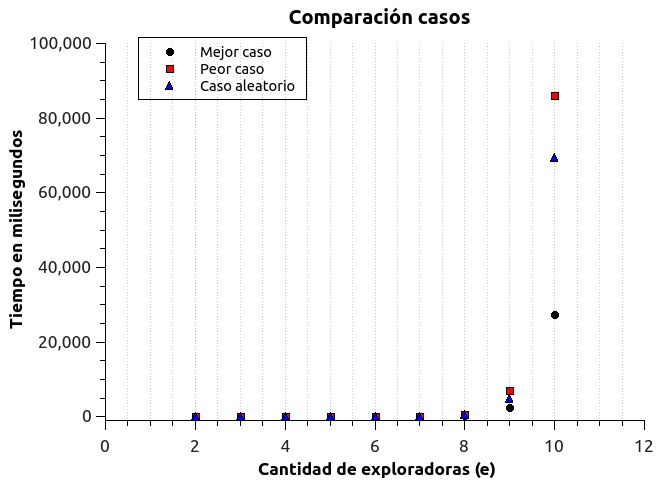
\includegraphics[width=\linewidth]{../graficos/ej3/ComparacionCasos.png}
  \caption{{\small Comparación de los mejores y peores casos para cada tamaño de entrada. También incluimos casos aleatorios.}} \label{asd}
\endminipage

\end{center}
\end{figure} 

Los mejores casos son aquellos en los que las exploradoras tienen solo una amiga cada una, pues a la hora de calcular las distancias, hay menos amistades que sumar a la suma total. Al contrario, los peores casos son aquellos en los que todas las exploradoras son amigas con todas. Damos un ejemplo de peor y mejor caso para un ronda de 6 exploradoras: \\
a bcdef (mejor caso) \\
a bcdef;b cdef;c def;d ef;e f (peor caso) \\
Las instancias de mejores y peores casos las generamos manualmente (ver Mejor$\_$PeorCaso.txt), mientras que para las de casos aleatorios hicimos un generador que utiliza la función $rand$ de c++ (ver generador.cpp). \\
Para apreciar mejor las diferencias entre los distintos casos hicimos el siguiente gráfico, que es un ``zoom"$ $ del anterior en las instancias más pequeñas.

\begin{figure}[H] 
\begin{center}

\minipage{0.8\textwidth}
  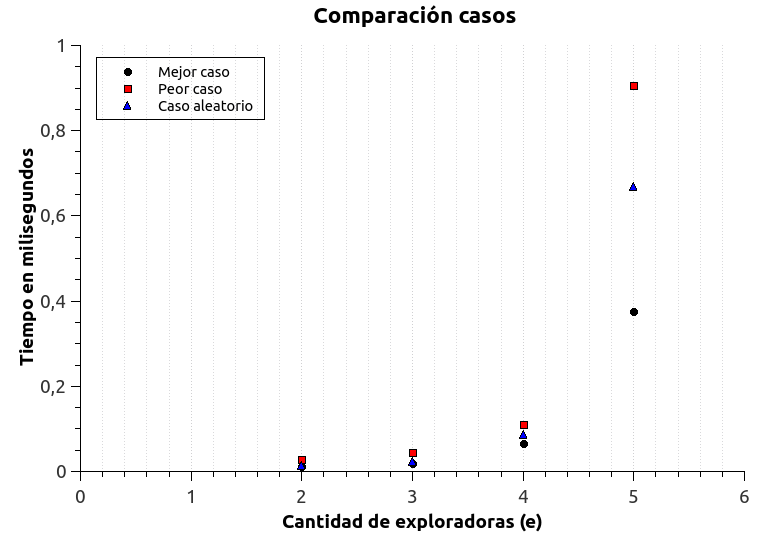
\includegraphics[width=\linewidth]{../graficos/ej3/ComparacionCasosZoom.png}
  \caption{{\small Comparación de los mejores y peores casos para cada tamaño de entrada. También incluimos casos aleatorios.}} \label{asd}
\endminipage

\end{center}
\end{figure}

Si bien en instancias de entrada pequeñas los tiempos de ejecución de la computadora son muy rápidos, de todas formas se puede ver la diferencia entre los distintos casos.

\begin{figure}[H] 
\begin{center}

\minipage{0.8\textwidth}
  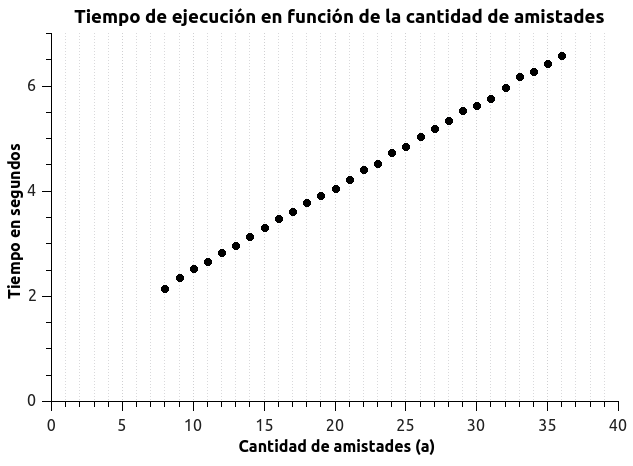
\includegraphics[width=\linewidth]{../graficos/ej3/CantidadAmistades.png}
  \caption{{\small Tiempo de ejecución en función de la cantidad de amistades en un grupo de 9 exploradoras.}} \label{asd}
\endminipage

\end{center}
\end{figure}

El gráfico recien expuesto nos muestra cómo aumenta el tiempo de ejecución en función de la cantidad de amistades del grupo de exploradoras. Para realizarlo, fijamos la cantidad de exploradoras en 9 (por eso los puntos comienzan en 8, pues es la mínima cantidad de amistades posibles) y fuimos agregando amistades hasta que ya no había ninguna por agregar. Este gráfico nos permite dar cuenta que la complejidad de nuestro algoritmo claramente depende de a.  

\begin{figure}[H] 
\begin{center}

\minipage{0.8\textwidth}
  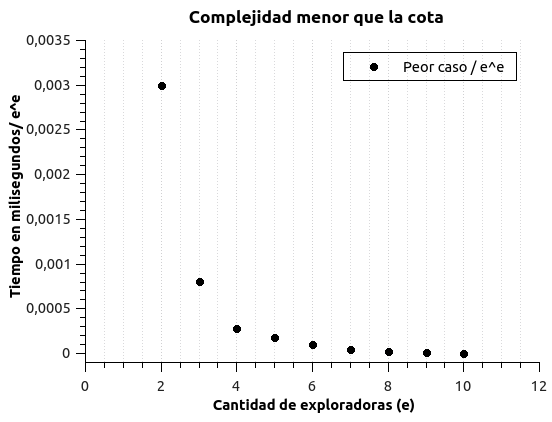
\includegraphics[width=\linewidth]{../graficos/ej3/ComplejidadCota.png}
  \caption{{\small Complejidad de nuestro algoritmo acotada por la del enunciado.}} \label{asd}
\endminipage

\end{center}
\end{figure}

En este gráfico dividimos los tiempos de los peores casos por e$^e$ y como la curva tiende a 0, concluimos que la complejidad de nuestro algoritmo es
menor que e$^e$.\\

Aclaración: en los archivos y carpetas de código se pueden ver muchos ejemplos para testeo.






\newpage
\section{Conclusión}
En este trabajo realizamos 3 algoritmos distintos que resuelven los ejercicios que nos presentaron, respetando la cota de complejidad dada. Explicamos cada algoritmo con ejemplos y pseudocódigos, analizamos la correctitud de ellos, demostramos que los mismos respetan dicha cota y los analizamos mediante tests de mejor y peor caso, y de casos random. Ilustramos estos resultados con gráficos. Para realizarlos, siempre que fue posible, tomamos el tiempo promedio de 100 ejecuciones del algoritmo para que el valor sea lo más representativo posible. \\
La etapa de experimentación, entre otras cosas, nos permitió sacar conclusiónes, entender mejor el funcionamiento de los algoritmos y darnos cuenta de no sólo dependían del tamaño de entrada, sino también de los valores de las mismas.   



%\newpage
%\section{Bibligraf\'ia y recursos}
%\input{bibliografia}

\end{document}
